
% % % % % % %  THE TEMPLATE TILL THE TITLE CAN BE USED AS IT IS%%%%%%%%%%%%%%%%%%%%%%%
% % % you are going to need revtex4-1 on your machine..........
\documentclass[prl,12pt,citeautoscript,reprint]{revtex4-1}
%\documentclass[preprint,12pt]{revtex4}
%\documentclass[preprint,12pt]{revtex4}
\usepackage{graphicx}
\usepackage{epsfig}
\usepackage{float}
\usepackage{amsmath}
\usepackage{graphicx}% Include figure files
\usepackage{dcolumn}% Align table columns on decimal point
\usepackage{bm}% bold math
\usepackage{amssymb}
\usepackage{amsmath}
\usepackage{epsf}
\usepackage{subfigure}
\usepackage{epstopdf}
\usepackage{color}

\usepackage{subeqnarray}
\usepackage{mathrsfs}
\usepackage[colorlinks=true, pdfstartview=FitV, linkcolor=red, citecolor=blue, urlcolor=blue]{hyperref}
\newcommand{\be}{\begin{equation}}%% begin equation
\newcommand{\ee}{\end{equation}} %% end equation
\newcommand{\ben}{\begin{eqnarray}} %% begin equation array
\newcommand{\een}{\end{eqnarray}} %%% end equation array




\usepackage{tikz}
\usetikzlibrary{shapes,arrows,positioning,calc}


\usepackage[colorlinks=true, pdfstartview=FitV, linkcolor=red, citecolor=blue, urlcolor=blue]{hyperref}
\begin{document}
\title{Modeling MSEIRS with deterministic differential equations model and cellular automaton model}
\author{Vaibhav Amit Patel (ID:201401222)}
\email{201401222@daiict.ac.in}
\author{Tanmay Patel (ID:201401409)}
\email{201401409@daiict.ac.in}


\affiliation{CS-302 Modeling and Simulation course, DA-IICT}


\begin{abstract}
We try to model the MSEIRS epidemic model with cellular automaton. MSEIRS model is used when there is passive immunity from the mother and the recovered can become infectious again. After using different initial conditions as seed we try to get the same behaviour as the differential equations’. We will discuss about the basic reproduction number and initial conditions of the automaton. The disease that is taken under consideration is pertussis (whooping cough).
\end{abstract}
\maketitle
\section{Introduction}
Epidemic spread of different infectious diseases have been modeled by many researchers. After making these models, these models can be applied to relevant diseases. SIR model is the basic and the first most popular version of epidemic spread model \cite{kermack1927contribution}. In this paper, Kermack et. al. showed mathematical details of the SIR model and more. Johnson \cite{johnson2009mathematical}, this paper explains the details, assumptions and other small details in an easy way. After this basic model, there are many different variants of this model are available and studied for different assumptions to include in the modeling  \cite{allen1994some,korobeinikov2004lyapunov,jin2007sirs,li1995global,anguelov2009comparison} . These models include SIR model with births and deaths, SEIS model, SEIR model, MSIR model, MSEIR model etc. 
\par 
The MSEIRS model includes the case when an individual is born with natural passive immunity, specifically maternal passive immunity. In the maternal passive immunity, either the fetus is born with immunity or it gets immune with breast feed of the human milk. These disease includes immunity in Hepatitis B, polio, TB, Pertussis(Whooping cough) etc. But, in the MSEIRS model the recovered can become susceptible again. In the real world Hepatitis B and other disease can not happen again. That is why we are considering Pertussis disease in our discussion. The parameters are estimated by keeping the disease in mind. A person with whooping cough can infect another person when he breathes, sneezes or coughs. The disease can be cured with vaccine. It is a highly contagious infection.

\section{Model}
We model this problem in \begin{enumerate}
    \item Deterministic compartment model
    \item Cellular automaton.
\end{enumerate}
First, we will discuss the deterministic compartment model. 
Here, we are considering standard assumption of the epidemic compartment model.
M(t) denotes the number of people with maternal passive immunity. B is the birth rate for infants. In all the equations, $\mu{_1}$ is the death rate for non-infecteds, which depends on the population. An immune can become susceptible with the rate $\delta$.    
$$\frac{dM}{dt} = B -(\delta - \mu{_1}) M$$
S(t) denotes the susceptible, the number people who can become infected due to contact of any infected person, but not became infected yet. Here, the inflow term is simply the immune becoming susceptible term and outflow terms include death rate and the interaction term. The interaction term depends on the number of susceptible and infected multiplied by the term $\beta$, which is the rate at which this interaction makes the susceptible quarantined. 
$$\frac{dS}{dt} = B + \delta M -\frac{\beta S I}{N} - \mu{_1} S + \rho R$$
% Define block styles
\tikzstyle{decision} = [diamond, draw, fill=blue!20, 
    text width=4.5em, text badly centered, node distance=3cm, inner sep=0pt]
\tikzstyle{block} = [rectangle, draw, fill=blue!20, line width=0.5mm,
    text width=3em, text centered, rounded corners, minimum height=2em]
\tikzstyle{line} = [line width=0.5mm,draw, -latex']
\tikzstyle{cloud} = [draw, ellipse,fill=red!20, node distance=3cm,
    minimum height=2em]
\tikzstyle{myarrows}=[line width=1mm,draw=blue,-triangle 45,postaction={draw, line width=3mm, shorten >=4mm, -}]


\begin{figure}[H]    
\begin{center}

\begin{tikzpicture}[node distance = 2cm, auto]
    % Place nodes
    \node [block] (M) {\bf M};
    \node [block, below=1.3 cm of M] (S) {\bf S};
    \node [block, below=1.3 cm of S] (E) {\bf E};
    \node [block, below=1.3 cm of E] (I) {\bf I};
    \node [block, right=1.3 cm of S] (R) {\bf R};


    %% Draw edges

    
    \path [line] (R) -- node[] {$\bm{\rho}$} (S);
    \path [line] (M) -- node[] {$\bm{\delta}$} (S);
    \path [line] (S) -- node[] {$\bm{\beta}$} (E);
    \path [line] (E) -- node[] {$\bm{\epsilon}$} (I);
    \path [line] (I.east) -- node[below=7pt] {$\bm{\gamma}$} (R);

    
\end{tikzpicture}

 \caption{\textbf{Combined network}}
  \label{fig:arcc}
  \end{center}

\end{figure}


E(t) denotes the number of people in the quarantined state i.e. The number of people that are in the latent period of the disease. Here, the inflow term is coming from the susceptibles and the outflow is death with rate $\mu{_2}$ and going into infected category with the rate $\epsilon$. Here $\mu{_2}$ is greater than $\mu{_1}$ because we have assumed that death rate of infected as well as people in latent period of disease is higher than normal death rate.
$$\frac{dE}{dt} = \frac{\beta S I}{N} - (\epsilon + \mu{_2}) E$$
I(t) denotes infected, the number of people that can infect the susceptible person, when come in contact. These people themselves are infected with the disease. They are the spreaders of the infectious disease. An infected can recover or dead with rate $\gamma$ and $\mu{_2}$ respectively. 
$$\frac{dI}{dt} = \epsilon E - (\gamma + \mu{_2})I$$
R(t) is the recovered category, the number of people that are removed from the infected category due to recovery from the disease. As the name suggests, it is MSEI\textbf{RS} model and that is why the recovered can become susceptible again. 
$$\frac{dR}{dt} = \gamma I - (\mu{_1} + \rho) R$$

\begin{table}[H]
    \centering
     \begin{tabular}{|c|c|c|} 
\hline
Parameter & Explanation & Value\\[0.7ex] 
 \hline
 $B$ & Birth rate per day & 10 \\ 
 \hline
 $\delta$ & Passive immune becomes& 0.005 (200 days) \\ 
  & susceptible rate &  \\ 
 \hline
 $\mu{_1}$ & Death rate & 0.002 \\ 
 \hline
 $\mu{_2}$ & Death rate for infecteds& 0.007 \\ 
  &and exposed&  \\ 
 \hline
 $\beta$ & A susceptible meets  & 0.6 \\ 
  & an infected at contact  & \\
  &rate of 10 it can go in latent& \\ 
  &period with probability 0.06 &  \\ 
 \hline
 $\epsilon$ & Quarantined becomes infected & 0.071 (14 days) \\ 
 \hline
  $\gamma$ & Infected gets recovered & 0.0667 (15 days) \\ 
 \hline

 $\rho$ & Recovered becomes & 0.001  \\ 
 &susceptible again &(1000 days) \\ 
 \hline
 
 \end{tabular}
    \caption{\textbf{Parameters used in the simulation}}
    \label{tab:tab_2}
\end{table}

\par Now, we will describe the cellular automaton model. The rules for the automaton are given below. Note that, it is not an exhaustive list of all the rules. The ones which are obvious from the deterministic model are not explicitly listed.
\begin{enumerate}
    \item The most interesting term in the former model was the interaction term ($\beta SI$). All the infectious neighbour of a susceptible individual can infect the susceptible with the probability $ \frac{\beta}{10}$. $\beta$ is the product of the contact rate and probability that the susceptible becomes the infected. The contact rate is 10, that is why the probability is $\frac{\beta}{10}$.
    \item A passive immune becomes susceptible again after some days, say x. To accommodate it in the automaton, a time step counter of each position was maintained. After 60 time stamps a passive immune will become susceptible.
    \item Quarantined becomes infected in $\epsilon^{-1}$ days. By using the same logic in the above rule, after 14 times stamps of being in the state of quarantine an individual becomes an infected.
    \item To include natural death in the model, each cell, at every time stamp, irrespective of the its state can die with probability 0.002.
    \item To include birth in the model, we have to have some position where the infant can be added. That is why, the dead state is made available. A dead state can become alive (of course another individual) with probability 0.002.
    \item The model includes the constant birth rate, using a probability that a dead cell can become alive with probability 0.002 and it becomes passive immune or susceptible. 
\end{enumerate}
\subsection{Reproduction number}
Reproduction number is defined as the expected number of secondary infectious cases resulting from an average infectious case once the disease has started to spread. 

In this model, it can be seen as the product of number of contacts per day that results into infection (${\beta}$) and average period of infection ($\frac{1}{\gamma + \mu{_2}}$). 
$$R{_0} = \frac{\beta}{\gamma + \mu{_2}}$$

\section{Results}
\begin{figure}[H]
\begin{center}
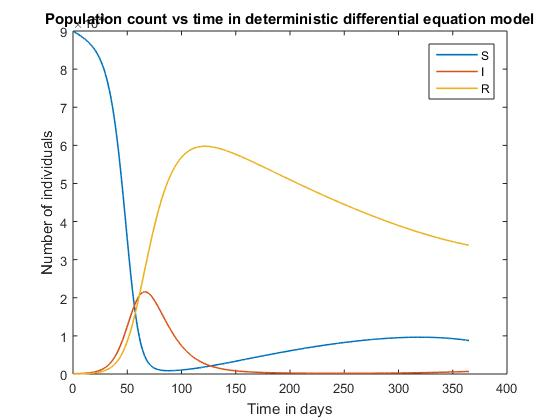
\includegraphics[scale=0.33]{n1}
\begin{minipage}{0.45\textwidth} 
{\footnotesize As we can see, the model is giving the expected results. The epidemic settles after 150 days. The number of infected do not die off because it receives a supply of susceptibles from the recovers. The number of infecteds decreases and increases after sometime because after sometime the recovers to susceptible conversion kicks in.

\par}
\end{minipage}
 \caption{\textbf{deterministic differential equation model}}
  \label{fig:bn}
\end{center}
\end{figure}


\begin{figure}[H]
\begin{center}
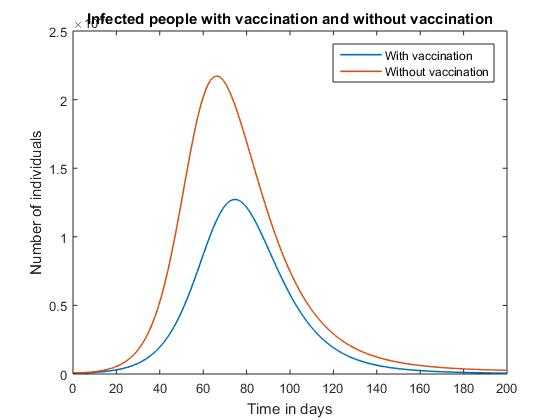
\includegraphics[scale=0.33]{n3}
\begin{minipage}{0.45\textwidth} 
{\footnotesize  The results are obvious from conditions. Vaccination tries to stop the epidemic, from the time it applied.
\par}
\end{minipage}
 \caption{\textbf{Infected people with and without vaccination}}
  \label{fig:bn}
\end{center}
\end{figure}

\begin{figure}[H]
\begin{center}
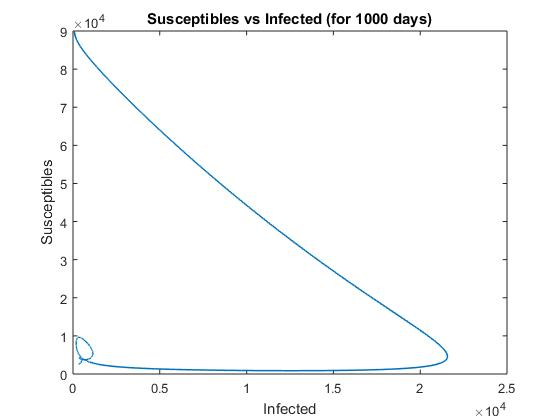
\includegraphics[scale=0.33]{n2}
\begin{minipage}{0.45\textwidth} 
{\footnotesize  From the initial condition and simulation results, we observe that the phase plot starts at the upper left point and ends at the other end in the bottom left part. The curve at the bottom is the time when the recovereds to susceptible part comes in the picture.
\par}
\end{minipage}
 \caption{\textbf{Phase plot of the Suscepibles and Infecteds}}
  \label{fig:bn}
\end{center}
\end{figure}



\begin{figure}[H]
\begin{center}
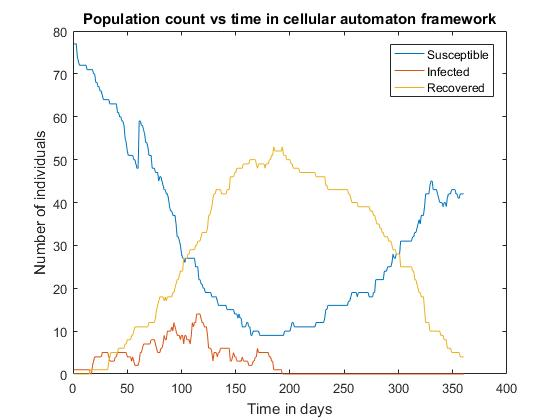
\includegraphics[scale=0.33]{im2}
\begin{minipage}{0.45\textwidth} 
{\footnotesize The results are giving same behaviour as in the deterministic compartment model (FIG. 2.) . It has stochastic properties, because the automaton do not have the information of the whole grid. It only has local properties. That is why the curve is not smooth. 
\par}
\end{minipage}
 \caption{\textbf{Population of vs time stamps in the Cellular automaton framework}}
  \label{fig:bn}
\end{center}
\end{figure}

\begin{figure}[H]
\begin{center}
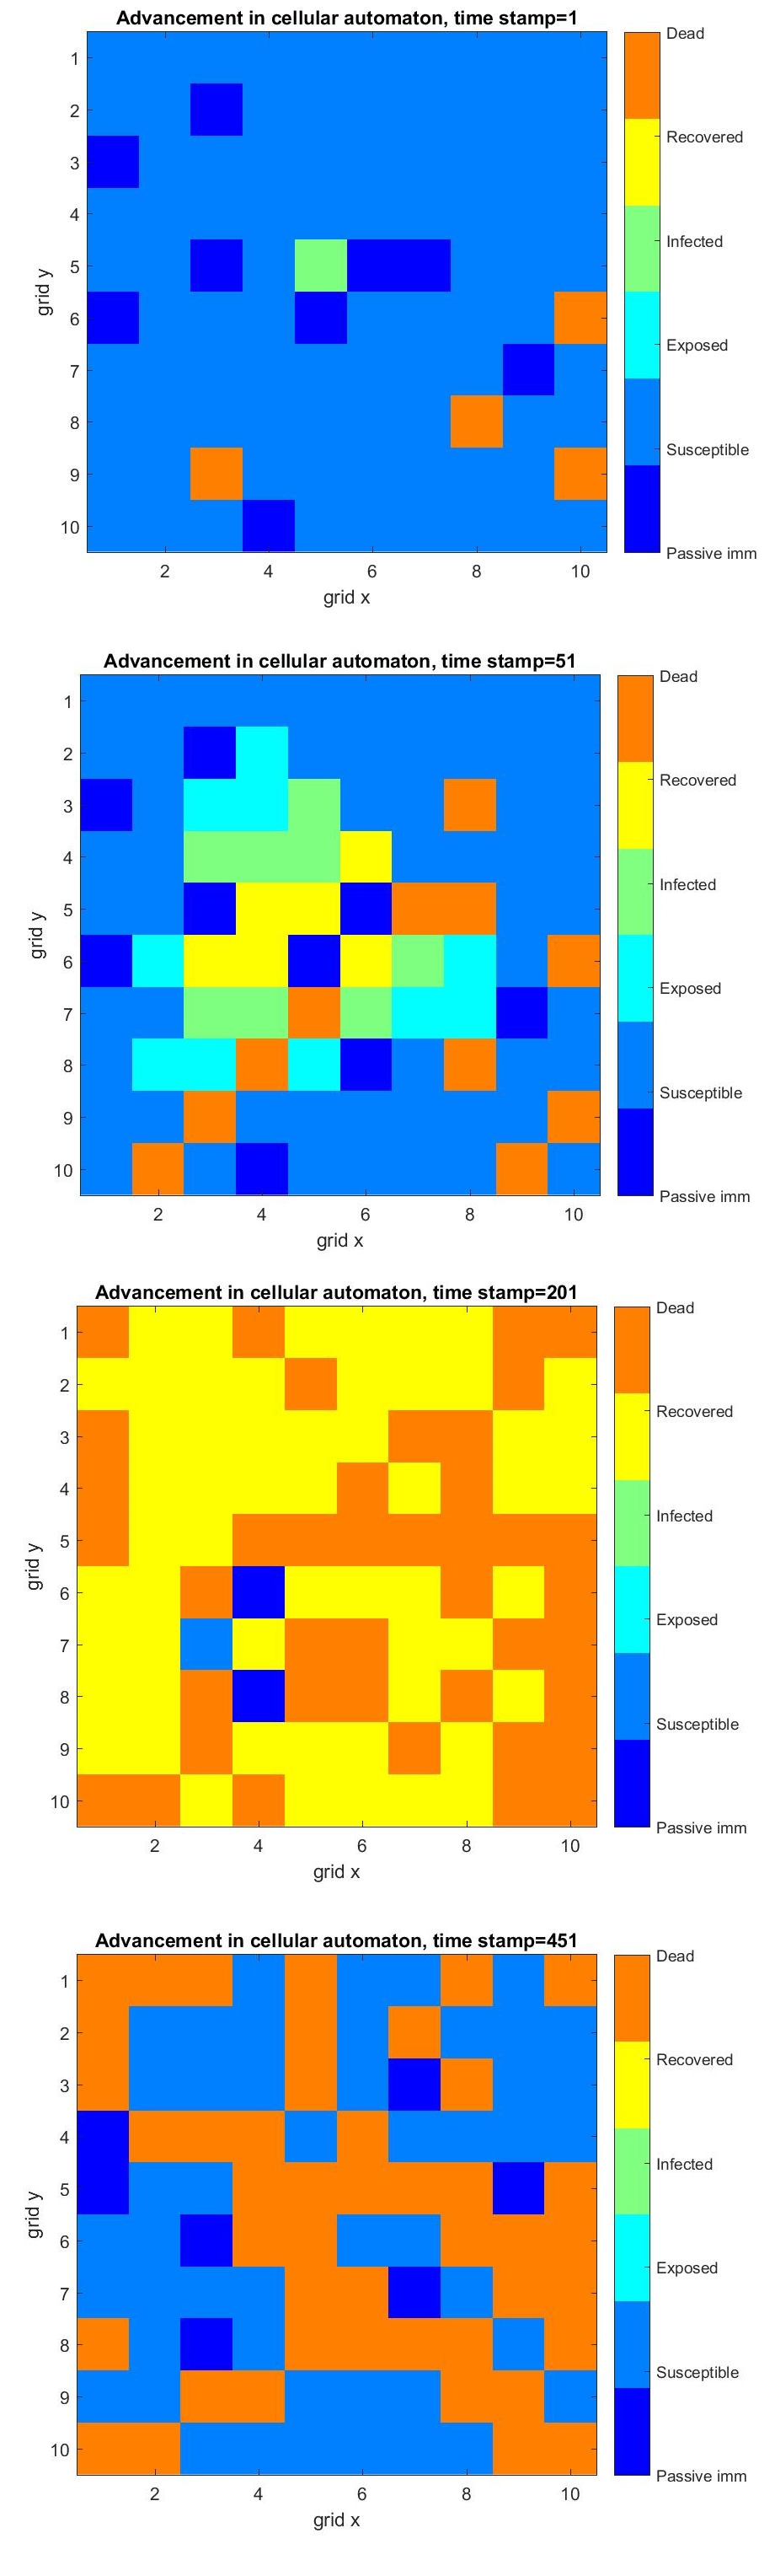
\includegraphics[scale=0.26]{fin}
\begin{minipage}{0.45\textwidth} 
{\footnotesize In this figure, we can see the states of all the positions in the study at some selected time stamps. \textbf{(1)} The grid is randomly initialized  in space with 1 infected, 9 passive immunes, 4 dead (no one) and others were susceptibles. \textbf{(2)} After some times the spread of the infection happens.
 \textbf{(3)} Then mostly the recovereds and dead remains.
 \textbf{(4)} After many time stamps, the recovereds become susceptible again and at the blank positions, either passive immune or susceptibles born. The video is included here: \url{https://drive.google.com/file/d/0B8QUo9TGO7EgVEY3WTdtRVVxbTg/view?usp=sharing}. 

 \par}
\end{minipage}
 \caption{\textbf{Advancement in the grid at different time stamps}}
  \label{fig:bn}
\end{center}
\end{figure}



\section{Conclusion}
In this work, we have modeled pertussis disease with the MSEIRS model. The model was trained using both, the deterministic approach and the cellular automaton. The epidemic eventually dies away. 
In the model, we have tried to include all the setting that the deterministic model provides. But some things which do not depend on the local property, but depend on the overall number of people in the study, can not be included in the cellular automaton. In the FIG. 5.(4) we can see that the model can not include the fact that there are no people other than suscpetible in the spatial world, but it remain producing passive immunes. The rules for the automaton were good enough to produce the same results as in the deterministic model.

\nocite{*}
  \bibliographystyle{acm}
\bibliography{sample}
\end{document}